% Source: Wald GR, physical PDF p. 157
%         (printed p. 144).
% Coverage: Figure 6.6, bending of light.
% Figures/tables/footnotes: Figure 6.6; no tables or footnotes.
% Status: source-reviewed and compile-clean.
% Uncertainties: none.
\begingroup
\renewcommand{\thefigure}{6.6}
\begin{figure}[htbp]
\centering
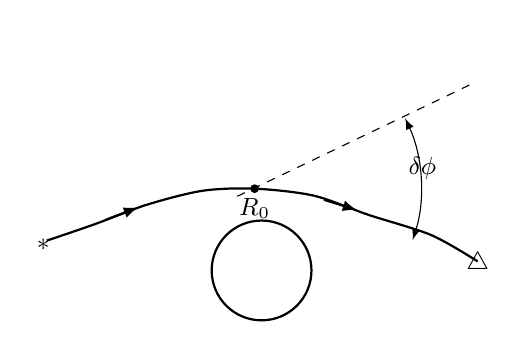
\begin{tikzpicture}[scale=.88,>=latex,font=\small]
  \draw[thick] (0,-.35) circle (.72);
  % Tangent to the ray at closest approach; its angular separation from the
  % outgoing asymptote is the deflection angle.
  \draw[dashed] (-.35,.72) -- (3.05,2.35);
  \draw[thick,smooth] plot coordinates {
    (-3.1,.08) (-2.4,.32) (-1.65,.60) (-.85,.80) (-.10,.83)
    (.75,.73) (1.55,.45) (2.45,.16) (3.12,-.22)};
  \draw[->,thick] (-2.25,.38) -- (-1.78,.56);
  \draw[->,thick] (.90,.67) -- (1.38,.52);
  \fill (-.10,.83) circle (1.8pt) node[below] {\(R_0\)};
  \node at (-3.15,.02) {\(\ast\)};
  \node at (3.12,-.24) {\(\triangle\)};
  \draw[<->] (2.18,.09) arc[start angle=-18,end angle=25,radius=2.40];
  \node at (2.32,1.12) {\(\delta\phi\)};
  % Reserve trim clearance above the artwork when this float lands at page top.
  \path[draw=none] (0,3.15) circle[radius=.1pt];
\end{tikzpicture}
\caption{Diagram illustrating the bending of light effect.}
\label{fig:6.6}
\end{figure}
\endgroup
